\def\mytitle{MATRICES USING PYTHON}
\def\myauthor{V.GOKULKUMAR}
\def\contact{velicharlagokulkumar@gmail.com}
\def\mymodule{Future Wireless Communication (FWC)}
\documentclass[10pt, a4paper]{article}
\usepackage[a4paper,outer=1.5cm,inner=1.5cm,top=1.75cm,bottom=1.5cm]{geometry}
\twocolumn
\usepackage{graphicx}
\graphicspath{{./images/}}
\usepackage[colorlinks,linkcolor={black},citecolor={blue!80!black},urlcolor={blue!80!black}]{hyperref}
\usepackage[parfill]{parskip}
\usepackage{lmodern}
\usepackage{tikz}
	\usepackage{physics}
%\documentclass[tikz, border=2mm]{standalone}
\usepackage{karnaugh-map}
%\documentclass{article}
\usepackage{tabularx}
\usepackage{circuitikz}
\usetikzlibrary{calc}
\usepackage{amsmath}
\usepackage{amssymb}
\renewcommand*\familydefault{\sfdefault}
\usepackage{watermark}
\usepackage{lipsum}
\usepackage{xcolor}
\usepackage{listings}
\usepackage{float}
\usepackage{titlesec}
\providecommand{\mtx}[1]{\mathbf{#1}}
\titlespacing{\subsection}{1pt}{\parskip}{3pt}
\titlespacing{\subsubsection}{0pt}{\parskip}{-\parskip}
\titlespacing{\paragraph}{0pt}{\parskip}{\parskip}
\newcommand{\figuremacro}[5]{
    \begin{figure}[#1]
        \centering
        \includegraphics[width=#5\columnwidth]{#2}
        \caption[#3]{\textbf{#3}#4}
        \label{fig:#2}
    \end{figure}
}
\newcommand{\myvec}[1]{\ensuremath{\begin{pmatrix}#1\end{pmatrix}}}
\let\vec\mathbf
\lstset{
frame=single, 
breaklines=true,
columns=fullflexible
}

\thiswatermark{\centering \put(181,-119.0){
\includegraphics[scale=0.13]{iith_logo3}} }
\title{\mytitle}
\author{\myauthor\hspace{1em}\\\contact\\FWC22034\hspace{6.5em}IITH\hspace{0.5em}\mymodule\hspace{6em}ASSIGN-5}
\date{}
\begin{document}
	\maketitle
	\tableofcontents
   \section{Problem}
   ABCDE is a pentagon. A line through
B parallel to AC meets DC produced at F. Show
that \\
(i) ar (ACB) = ar (ACF) \\       
(ii) ar (AEDF) = ar (ABCDE)

	    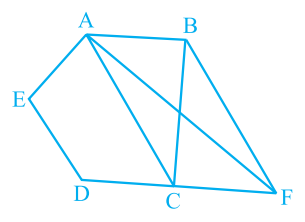
\includegraphics[scale=1.0]{diag_1.png}
   \section{Solution}
   \textbf{Theory:}\\
In pentagon ABCDE, $ AC\: || \: BF$ \\
\textbf{To Prove:} Ar(ACB)=Ar(ACF) \\
$\Delta$ ACB and $\Delta$ ACF lies on same base AC and are between same parallel AC and BF\\
\textbf{Theorem} : Two triangles on the same base (or equal bases) and between the same parallels are equal in area.
\begin{center}
$\therefore$ Ar($\Delta$ ACB)=Ar($\Delta$ ACF)......(1)\\
Hence, Proved    
\end{center}
\textbf{To Prove:}  Ar(AEDF)=Ar(ABCDE)\\
Add Ar(AEDC) to (1) both sides\\
Ar($\Delta$ACB)+Ar(AEDC)=Ar($\Delta$ACF)+Ar(AEDC)
\begin{center}
$\therefore$ Ar(ABCDE)=Ar(AEDF)     \\
Hence, Proved \\
\
\\
\
\\
\end{center}
\textbf{termux commands :}
\begin{lstlisting}
python3 matrix.py
\end{lstlisting}


The input parameters for this construction are 
\begin{center}
\begin{tabular}{|c|c|c|}
	\hline
	\textbf{Symbol}&\textbf{Value}&\textbf{Description}\\
	\hline
	a&6&AC\\
	\hline
	d&-3&DC\\
	\hline
	f&3&CF\\
	\hline
	$\theta$& 2$\pi/3$&$ \angle $C\\ 
	\hline
	C&$\
	\begin{pmatrix}
		0 \\
		0 \\
	\end{pmatrix}$%
	&Point C\\
	\hline
		E&$\
	\begin{pmatrix}
		-5 \\
		3 \\
	\end{pmatrix}$%
	&Point E\\
	\hline
\end{tabular}
\end{center}
\textbf{To Prove:} Ar(ACB)=Ar(ACF)
  %	\begin{align}
	%		\vec{C} &= \myvec{0 \\ 0}, \vec{E}=\myvec{-5 \\ 3}\\
	%			\vec{F} &= \myvec{3 \\ 0}, \vec{D}=\myvec{-3 \\ 0}
	%	\end{align}
		\begin{center}
	B= F-C+A\\
	Area of the triangle $\Delta$ACB is given by \\
Ar($\Delta$ACB) =$\frac{1}{2}$$\norm{\vec{A}\times\vec{B}}$............(2)\\
		Area of the triangle $\Delta$ACF is given by \\
 Ar($\Delta$ACF) =$\frac{1}{2}$$\norm{\vec{A}\times\vec{F}}...............(3)$
	\end{center}
	\textbf{To Prove:}  Ar(AEDF)=Ar(ABCDE)\\
	v1=E-A\\
	v2=E-D\\
	Ar($\Delta$AED)= 	$\frac{1}{2}$$\norm{\vec{v1}\times\vec{v2}}$..............(5)\\
	v3=D-A\\
	v4=D-C\\
	Ar($\Delta$ADC)= $\frac{1}{2}$$\norm{\vec{v3}\times\vec{v4}}$................(6)\\
	\begin{center}
	 		Ar(AEDC)=Ar($\Delta$AED)+Ar($\Delta$ADC)\\
	\end{center}
	\begin{center}
$\therefore$ Ar(AEDF)=Ar(AEDC)+Ar($\Delta$ACF)........(7)\\
$\therefore$ Ar(ABCDE)=Ar(AEDC)+Ar($\Delta$ACB).......(8)\\	\end{center}
The below python code realizes the above construction:	
\begin{lstlisting}
https://github.com/velicharlagokulkumar/FWC_module1/tree/main/matrices/lines/codes/matrix.py
\end{lstlisting}
 \section{Construction}
 	\begin{center}
  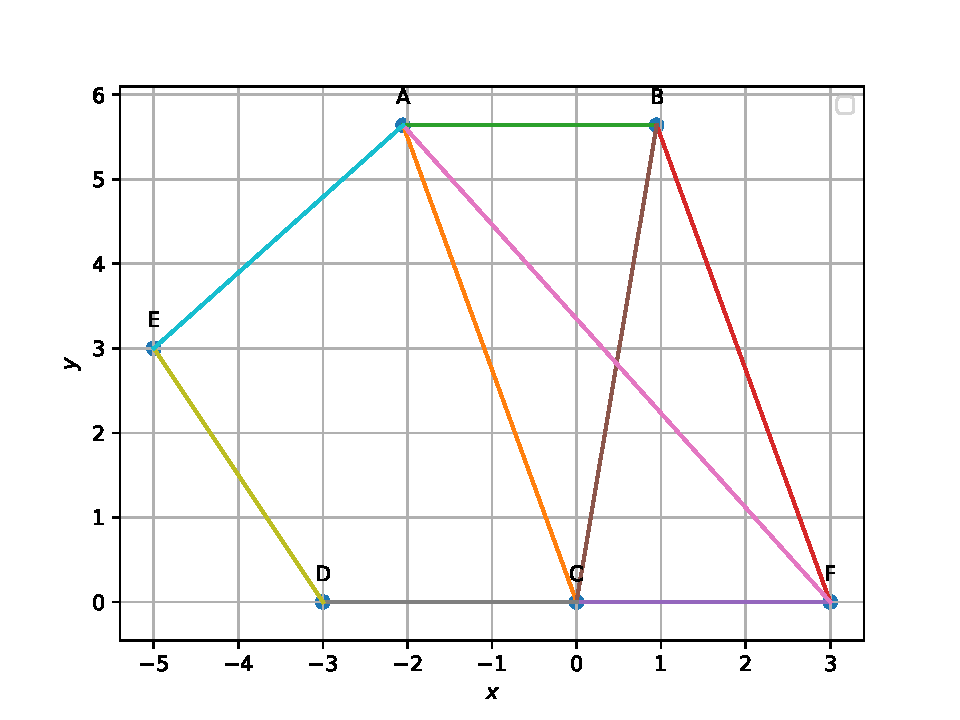
\includegraphics[scale=0.46]{matrix.pdf}
  	\end{center}
\bibliographystyle{ieeetr}
\end{document}